\chapter{Analysis and Design}

\section{Introduction} % Section 3.1
This chapter will present the analysis and design porition of the project. Identified are the system users and their needs, which are then translated into technical requirements, and finally the system's functional and architectural design is described. Several diagrams are included to aid with visualising the behaviour, workflow, and structure of the system.

\section{User Needs and Requirements} % Section 3.2
When developing any technology it is imperative to have a solid foundation upon which to build on and refer to throughout the development process. It should help provide a clear understanding of the problem, the needs expectations of the people who will be using it, and give some insight into how the original problem will be solved in the implementation stage. In the case of this project, the users include nurses and doctors, and the patients who will be using the device. There are several different users each with different required levels of control and functionalities, therefore it is crucial to translate their needs into measurable and clearly defined requirements that will steer the design and eventually implementation of the system.

The following pages present two key tables accomplishing that task: the \textbf{User Needs table} which outlines the what is required of the system by the users to solve their problem, and the \textbf{User Requirements table} which turns those needs into specific, quantifiable, and actionable requirements for the system to fulfil.

\begin{landscape}
\thispagestyle{empty}
\begin{table}[H]
\centering
\caption{User Needs Table}
% \begin{tabularx}{\linewidth}{|p{2.5cm}|p{15cm}|p{1.5cm}|}
\begin{tabularx}{\linewidth}{|p{2.5cm}|X|p{2cm}|}
\hline 
\textbf{ID} & \textbf{Description } & \textbf{Source} \\
\hline
UN-01 & Accurate capture of data from various medical devices in order to monitor patient status & Arduino \\
\hline
UN-02 & Simple pairing of the device to other medical devices through Bluetooth in order to easily setup and guarantee reliable data transfer & Arduino \\
\hline
UN-03 & Updating/setting of limits/conditions for different measurement types in order to customise each device to a particular patient's needs & Arduino/\newline Cloud/\newline Medical staff \\
\hline
UN-04 & Process data according to preset conditions in order to send only relevant data to the cloud & Arduino \\
\hline
UN-05 & Storing of data in the short-term in the case of high network congestion to prevent loss. (Only store after processing if values are abnormal/relevant to be sent to the cloud) & Arduino \\
\hline
UN-06 & Alert medical staff of patient status if critical or abnormal reading gathered in order to allow them to check on said patient in person & Cloud \\
\hline
UN-07 & Alert users about device status in order to allow them to keep it in a state where it is running normally & Arduino \\
\hline
UN-08 & Provide a general picture about the patient's status daily in order to track it over time (daily averages viewed in context of weeks, months, years) & Cloud \\
\hline
\end{tabularx}
\label{tab:user_needs_table}
\end{table}
\end{landscape}

\clearpage
\pagestyle{empty}
\begin{landscape}
% \begin{table}[H]
% \centering
\begin{longtable}{|p{2cm}|>{\RaggedRight\arraybackslash}p{6cm}|>{\RaggedRight\arraybackslash}p{6cm}|>{\RaggedRight\arraybackslash}p{6cm}|p{2cm}|}
\caption{User Needs Table}
\label{tab:user_requirements_table} \\
\hline 
\textbf{Req. ID} & \textbf{User Requirement Name} & \textbf{Description} & \textbf{Justification/Comment} & \textbf{Reference}\\
\hline
\endfirsthead

\hline
\textbf{Req. ID} & \textbf{User Requirement Name} & \textbf{Description} & \textbf{Justification/Comment} & \textbf{Reference}\\
\hline
\endhead

\hline
\endfoot

\hline
\endlastfoot

UR-01 & Temperature Reading & 5 times/12 hours\newline Accuracy: to nearest 0.1$^\circ$C & 5 readings in a single 12 hour period should be enough to detect any changes in temperature early enough after they get out of bounds & UN-01 \\
\hline
UR-02 & Blood Pressure Reading & 1 time/12 hours\newline Accuracy: $\pm$3mmHg for both systolic and diastolic & The recommended number of times to measure BP is once per day & UN-01 \\
\hline
UR-03 & Heart Rate Reading & 3 readings spaced 2 minutes apart / hour, and keeping the average of the 3 readings as final BPM value\newline Accuracy: $\pm$ 5 BPM & In a clinical/hospital environment there would be constant EKG measurement so there is no reason medically not to measure heart rate as often as possible. However to conserve battery, avoid network congestion, and keep the processor constantly working, 3 readings averaged on the hour is sufficient for this system & UN-01 \\
\hline
UR-04 & Bluetooth Pairing with Medical Devices & Visual interface to display BT connection status, and allow force disconnecting a device which has connected if it is not a medical device & Pairing with a device should be incredibly easy seeing as a likely user group will be elderly individuals & UN-02 \\
\hline
UR-05 & Per Vital Sign Configuration & Visual interface to be able to select a vital sign that will be measured, and set the upper and lower acceptable limits for it. This must persist across power loss and general restarting of the device. In addition, the limits must make sense in the context of the vital sign they relate to. For example it should be impossible to set an upper limit of 60$^\circ$C for temperature & Each patient has different medical needs and as such will need customised ranges for the acceptable readings. Furthermore, the patients should not be required to have to set these limits in the event of a power loss of the device or device restart & UN-03 \\
\hline
UR-06 & Data Processing and sending to the cloud & Process each data reading in the context of the device type's pre-set limits (lower/upper). Readings which are below/above the limits will be added to a queue. The front data will be sent to the cloud using the LoRaWAN protocol. Once confirmation is received that the data is successfully received, it will be dequeued and the next data (if it exists) will be transmitted. Allow up to 3 attempts before considering that there is a problem with the device/connection to the network and alerting the user. & Data that is within the acceptable limits does not need to be sent. The queue's purpose is to ensure any critical readings get to the cloud platform where the medical professionals can respond accordingly. & UN-04 \newline UN-05 \\
\hline
UR-07 & Notification of medical staff for abnormal reading & After sending data through the LoRaWAN protocol to the cloud, create some kind of notification for the medical staff in the form of of an email or "ticketing" system & A popup notification is not sufficient because it might be missed & UN-05 \newline UN-06 \\
\hline
UR-08 & Device status information & Constantly monitor device status (BT connection, state) and display this information to the user & Due to the fact that status information must always be visible, and we do not want to occupy the LCD screen with it all the time, the information will be available through coloured LED lights & UN-07 \\
\hline
UR-09 & Patient status tracking over time & Regardless of whether an abnormal reading is gathered, at fixed times of the day and for a set number of times, take readings and send them to the cloud even if they are not abnormal. & Patient history could be vital for providing medical staff with insight into the patient's condition, however there is no need to take more than one non-abnormal reading per day & UN-08 \\
\hline
\end{longtable}
% \end{table}
\end{landscape}

\clearpage

\section{System Behaviour and Workflow} % Section 3.3
\textbf{Note:} Diagrams need some tweaking before I can include them in here.

State diagram: Describing system states (DISCONNECTED, CONNECTED, SETUP, READING, PROCESSING, TRANSMITTING)

Use case diagram: Showing interactions between users (nurses, doctors, patients) and the system

Activity flowchart: Visualise workflow

\section{System Architecture and Design} % Section 3.4
\textbf{Note:} Diagrams need some tweaking before I can include them in here.

High-Level Architecture diagram: Overview of the system from the medical devices to the cloud with the BT module and arduino in the middle

Block diagram: Overview of circuit

\begin{figure}[H]
\centering
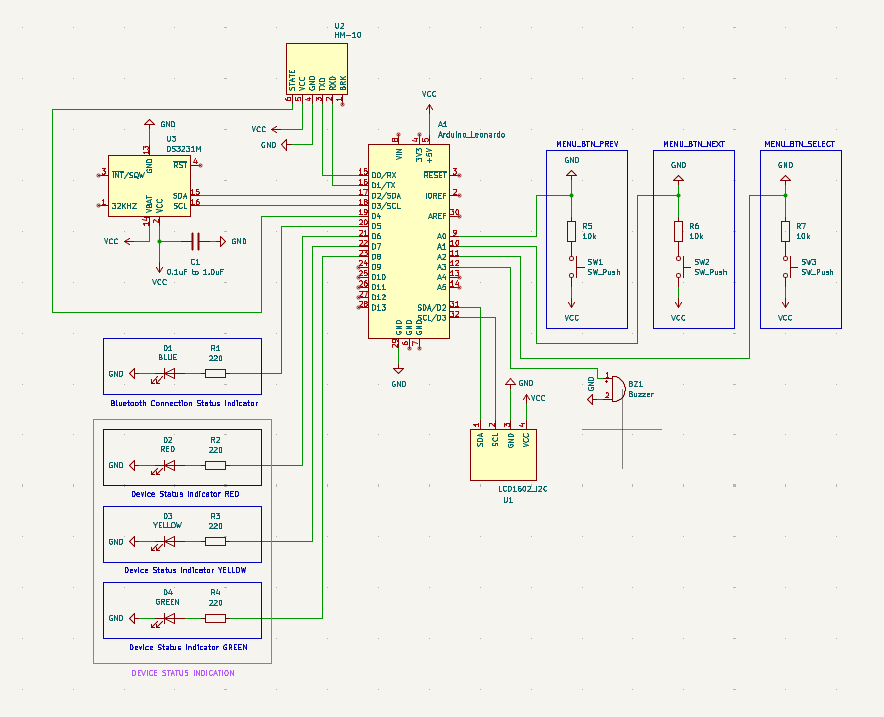
\includegraphics[scale=0.6]{images/schematic_rev2}
\caption{Detailed circuit shcemtatic of all all components in the device}
\label{fig:circuit_diagram}
\end{figure}

\section{User Interface Design} % Section 3.5
\textbf{Note:} Diagrams need some tweaking before I can include them in here.

Navigation Flow diagram: Show how a user might navigate around the device menus

Will discuss about usability and simplicity

\section{Project Planning} % Section 3.6
\textbf{Note:} Diagrams need some tweaking before I can include them in here.

Gantt chart here

Will discuss how project timeline led to certain design decisions being made

\section{Summary} % Section 3.7
This chapter expanded on the design of the system, starting from the user needs analysis, behaviour of the system, system architecture, and design of the interface. The provided diagrams show the organisation of the system, laying the foundation for the implementation which will be discussed in detail in the next chapter.
